% Chapter 1

\chapter{Introduction: What is a fractal?} % Main chapter title

\label{Chapter1} % For referencing the chapter elsewhere, use \ref{Chapter1} 

\lhead{Chapter 1. \emph{Introduction}} % This is for the header on each page - perhaps a shortened title

%----------------------------------------------------------------------------------------

Before we discuss multifractals, we begin with a discussion of normal, or mono-, fractals. We note the intuitive properties present in a simple example and how they differ from non-fractal geometry, and then \todo{This is probably going to be removed when the paper is changed to focus only on fractals and ignores multifractals.}

%----------------------------------------------------------------------------------------
\paragraph{An example of a fractal: the Koch snowflake (see Figure \ref{fig:kochcurve})}\label{fractalexample}\todo{rename this to reflect the inclusion of the Cantor set for comparison.}

\begin{figure}[h]
\centering
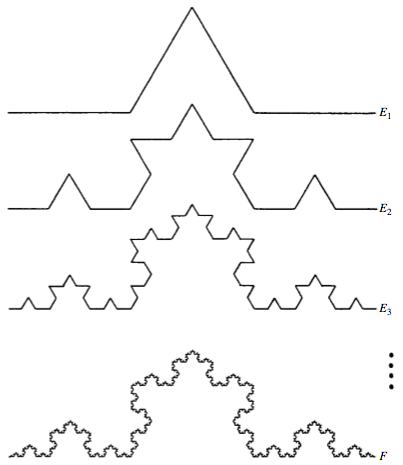
\includegraphics[height=0.6\textwidth]{Chapters/Figures/Kochcurve.png} 
\caption[Koch Curve]{Iterations of the Koch CURVE, a simple fractal exhibiting many characteristics typical of fractals. The initial figure at the top is made more and more textured with each iteration $E_{n}$, becoming rougher and more fractal-like as it approaches the final Koch curve $F$. Image credit: \citep{fractaltextbook}. }\label{fig:kochcurve}
\end{figure}

We note the most obvious properties of this fractal that separate it from a non-fractal shape. 
\textit{Its shape is defined recursively.} The Koch curve is a line segment on which an infinite number of iterations is performed as follows: each line segment in the $n$th iteration of the curve, having length $L_n$, is replaced by a scaled-down version of $E_1$ with length $4L_n/3$. This results in self-similarity at all scales: any section of the Koch curve contains an infinite number of repetitions of the original curve. 

\begin{myproposition} The length of the Koch curve is infinite. \end{myproposition}
\begin{myproof}
Because of the recursive rule defining the Koch curve, the curve's length is increased by a factor of $ 4/3 $ with each of the infinite iterations. We express the length of the curve after the $n$th iteration as $L_n$. The total length $L_\infty$ can be expressed as an infinite geometric sequence with a common ratio of $ 4/3 $:
\begin{equation}
	L_\infty = \lim_{n \to \infty}L_n = \lim_{n \to \infty}\left(\frac{4}{3}\right)^n L_0
\end{equation}.
Limits are linear with respect to multiplication by a constant, so we find:
\begin{equation}
	\lim_{n \to \infty}L_n = L_\infty = L_0 \lim_{n \to \infty} \left(\frac{4}{3}\right)^n
\end{equation}
which clearly increases without bound.\todo{Do I need to show this any more clearly?}
\begin{equation}
	\lim_{n \to \infty}L_n = \infty 
\end{equation}
The length of the Koch curve is thus infinite.
\end{myproof}

Area, another property of shapes in non-fractal geometry, is likewise not useful in describing the Koch curve: though we see that the additional length added with each iteration expands the fractal's size in the plane, the added segments have no thickness, and the area filled by the curve is thus zero.



\paragraph{Another example of a fractal: the middle-third Cantor set (see Figure \ref{fig:cantorset})}

\begin{figure}[ht]
\centering
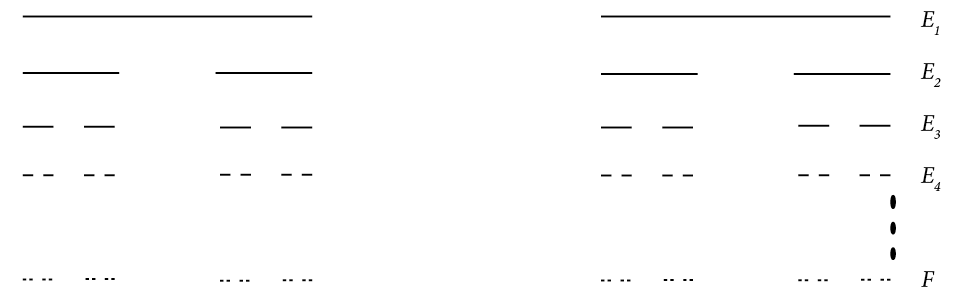
\includegraphics[width=0.9\textwidth]{Chapters/Figures/cantorset.png} 
\caption[Middle-third Cantor set]{}\label{fig:cantorset}
\end{figure}\todo{finish caption}




\todo{introduce the Cantor set and show why we need a fractal dimension}






Instead of classifying fractals by their length and area, then, we examine their ``roughness''. This, as we will discuss below, leads to the creation of different \textit{fractal dimensions} to classify the space-filling properties of these fractals.














\section{Fractal dimensions}

We use the word ``set" to more precisely refer to what might be simply called a shape; after all, every shape is just a set, possibly infinite, of points. As seen above, whereas non-fractal sets have well-defined, intuitively understood geometric properties such as length or area, fractal sets can be characterized by various concepts of dimension. Here, we will discuss \textit{box-counting dimension} in the greatest detail.

\subsection{Spaces, sets, and measures}

Before we venture further into classifying fractals by their dimension, we need the following definitions.

\begin{mydef}
We define an n-dimensional space $ \mathbb{R}^{n} $ to be the set of all points that can be identified by an ordered n-ple of real numbers. Hence, for example, any point $ \alpha $ in $ \mathbb{R}^{5} $ can be identified by the ordered 5-ple $ \alpha = (\alpha_{1}, \alpha_{2}, \alpha_{3}, \alpha_{4}, \alpha_{5})$ where $ \alpha_{1} ... \alpha_{5} \in \mathbb{R} $.\end{mydef}

We will now work by analogy to discuss the concept of a \textit{measure}\footnote{Analogy adapted from \citep{mandelbrotmultifractal}}. Consider a geographical map of some landmass, with a function $ \mu(\mathcal{S}) $ that denotes the volume of groundwater below any subset $ \mathcal{S} $ of the landmass. We note three intuitive properties of this measure $ \mu $:\begin{enumerate}
\item The measure of any subset of the space---or the volume of groundwater under any plot of land on the landmass---gives a numerical indication of the plot of land's magnitude. That is, it describes the plot's size when measured by groundwater content.
\item\label{measureofanullset} There should be no water under a plot of land with no size. 
\item\label{measureofsubsets} If a plot of land $ A $ contains another plot of land $ B $, there should be less or as much groundwater under $B$ as there is under $A$. 
\item\label{measureaddition} If we find the volume of groundwater under a plot of land on the landmass, we should get the same value or less than when we split the plot up into many pieces with overlap allowed and add up the volume of groundwater found under each piece. 
\end{enumerate}
We now formalize these properties below.

\begin{mydef}
We define a measure $ \mu $ to be a function on a space $ \mathbb{R}^{n} $ that assigns a positive number to each subset $ \mathcal{S} $ of $ \mathbb{R}^{n} $ such that:

\begin{itemize}
\item Because $\mu$ should characterize a set by its size in some sense, it is meaningless to have a nonzero size for any set with no elements. This is reflected in Property \ref{measureofanullset} above.
\begin{equation}
\mu(\emptyset) = 0
\end{equation}
\item The size of a set should be smaller than (or equal to, if $ A = B $, i.e., $B$ is not a proper subset of $A$) the size of a set that contains the first set and other elements too. This is reflected in Property \ref{measureofsubsets} above.
\begin{equation}
\mu(B) \le \mu(A) \mathrm{ \quad if \quad }  B \subset A.
\end{equation} 
\item The measure of a union of subsets should never be larger than the sum of the measures of the individual subsets: 
\begin{equation}
\mu\left(\bigcup_{i=1}^{\infty} A_i\right) \le \sum_{i=1}^{\infty} \mu(A_i) 
\end{equation}
Allowing for the measure of the union to be smaller than the sum of the individual measures accounts for overlap between the subsets; if, for all pairs of subsets $A_1$ and $A_2$, $A_1 \cap A_2 = \emptyset$, the measure of the union should be equal to the sum of the individual measures. In short, the measure should be distributive over addition.
\end{itemize}
We call the space on which the measure resides the \textit{support} of the measure.
\end{mydef}

\subsection{The dimension of a fractal}
Recall that in the example of the Koch curve above, we failed to usefully classify the shape by non-fractal means. Though we could see that the figure filled a space, we lacked language to discuss precisely how it filled that space; we could not quantify its ``roughness''. We introduce the box-counting dimension as a kind of analogy to the Euclidean dimension in order to quantify how a fractal set fills a space.

\subsubsection{What we mean by ``dimension''}\label{intuitivedimension}
Consider a line segment of length $ L_0 $. Note that when the segment is scaled by $\epsilon$, a number greater than one, into smaller pieces of equal size, each segment produced has length $L_0/\epsilon$. Now we repeat our exploration with a square of side length $ L_0 $. Here, when the square is scaled by a factor $\epsilon$, the smaller squares produced have an area $1/\epsilon^2$ the original. Again, when we repeat this procedure with a cube of side length $ L_0 $ we find that the cubes produced all have volumes $1/\epsilon^3$ the original. Hence, we generalize that the number of pieces $n$ produced from scaling by a factor of $\epsilon$ is given by 
\begin{equation}n = 1/\epsilon^D\end{equation}
where $D$ is the dimension of the shape, and we can now solve for dimension:
\begin{equation}\label{dimensionEqn} D = \frac{\log{n}}{\log{(1/\epsilon)}}\end{equation}

We now return to the Koch curve. We recognize the first iteration $E_1$ as the fundamental unit of all other iterations of the curve. That is, we can replace each of the four line segments that make up $E_1$ with a scaled-down copy of the original $E_1$ in order to reach the next iteration, and by repeating this process ad infinitum we can reach the final curve $F$. We can, however, view this process in the framework established in the example above, so that each iteration replaces one line segment with a length $L_0$ with four others, each of which has a length of $L_0/3$. This is akin to the method described above: our fractal produces $n = 4$ smaller pieces each time it is scaled, and each piece is $1/\epsilon = 1/3$ the size of the original. Hence, we can apply the equation for dimension (Equation \ref{dimensionEqn}) to the Koch curve:
\begin{equation}D = \frac{\log{n}}{\log{(1/\epsilon)}} = \frac{\log{4}}{\log{3}} \end{equation}

\begin{myremark}What does this dimension mean? Again, it seems intuitive that the dimension would be between one and two---this generalization of dimension should resemble the more familiar case of non-fractional dimensions, and the Koch curve is certainly greater than one-dimensional while not filling the entire plane as a two-dimensional shape would. \end{myremark}

\subsubsection{Box-counting dimension}
We now seek to formalize our understanding of dimension\footnote{``There is no one dimension that can only describe a fractal set; many different types of dimension exist, and all provide very different conceptions of a fractal's properties'' \citep{fractaltextbook}.} Furthermore, we wish to formalize this understanding in a way that allows us to discuss fractal objects that are not strictly self-similar\footnote{As mentioned in Section \ref{fractalbasics}, fractals are not as concretely defined as one would hope, and we tend only to classify a shape as a fractal when it possesses a reasonably large number of the fractal properties identified in Section \ref{fractalbasics}---when a shape has sufficient ``roughness'' that the language of fractal geometry becomes more useful in describing its characteristics.}. For this we introduce a specific dimension, the \textit{box-counting dimension}. In addition, the box-counting dimension is computationally much more simple than other fractal dimensions, such as the Hausdorff dimension \citep{fractaltextbook}.

The box-counting dimension gives an analogue of the dimension defined by Equation \ref{dimensionEqn}: the fractal set is covered by a number of cubes\footnote{A ``cube'' here is not strictly three-dimensional; the shape has analogues in all other dimensions as well.} with side length $\epsilon$. We extend the number of replacements $ n $ from Equation \ref{dimensionEqn} to take the smallest number of cubes that can cover the fractal set. The box-counting dimension is given by the limit of this extension of Equation \ref{dimensionEqn} as the side $\epsilon$ approaches zero.

\begin{mydef} We define the box-counting dimension of a fractal set $ F $, $\operatorname{dim}_B F $, as follows:
\begin{equation}\operatorname{dim}_B F = \lim_{\epsilon \to 0} \frac{\log N_\epsilon(F)}{-\log\epsilon}
\end{equation}
where $N_\epsilon(F)$ is the number of cubes of side-length $\epsilon$ that cover the fractal set $F$.
\end{mydef}

\begin{myexample}We can apply numerical techniques to verify the agreement of this definition with that established in Section \ref{intuitivedimension}. A computational module to calculate the box-counting dimension is included in \ref{AppendixA} and is here applied to a Koch curve of size ???? pixels end-to-end. ****include graphics of curve and results, compare dimensions and error****  \end{myexample}

\begin{myexample}Same thing, Sierpinski pyramid, perhaps?\end{myexample}

%	Should I extend this discussion? Include some implications and whatnot? Also, can/should I go back to Hausdorff? I need to get on with multifractals, I think.

\listoftodos






































